% TikZ and PGF 2.00
% Source: TikZ and PGF manual
\documentclass{standalone}
\usepackage{tikz}
\usetikzlibrary{shapes,decorations,shadows}
\usetikzlibrary{decorations.pathmorphing}
\usetikzlibrary{decorations.shapes}
\usetikzlibrary{fadings}
\usetikzlibrary{patterns}
\usetikzlibrary{calc}
\usetikzlibrary{decorations.text}
\usetikzlibrary{decorations.footprints}
\usetikzlibrary{decorations.fractals}
\usetikzlibrary{shapes.gates.logic.IEC}
\usetikzlibrary{shapes.gates.logic.US}
\usetikzlibrary{fit,chains}
\usetikzlibrary{positioning}
\usepgflibrary{shapes}
\usetikzlibrary{scopes}


\begin{document}


\tikzset{paint/.style={ draw=#1!50!black, fill=#1!50 },
    decorate with/.style=
    {decorate,decoration={shape backgrounds,shape=#1,shape size=2mm}}}

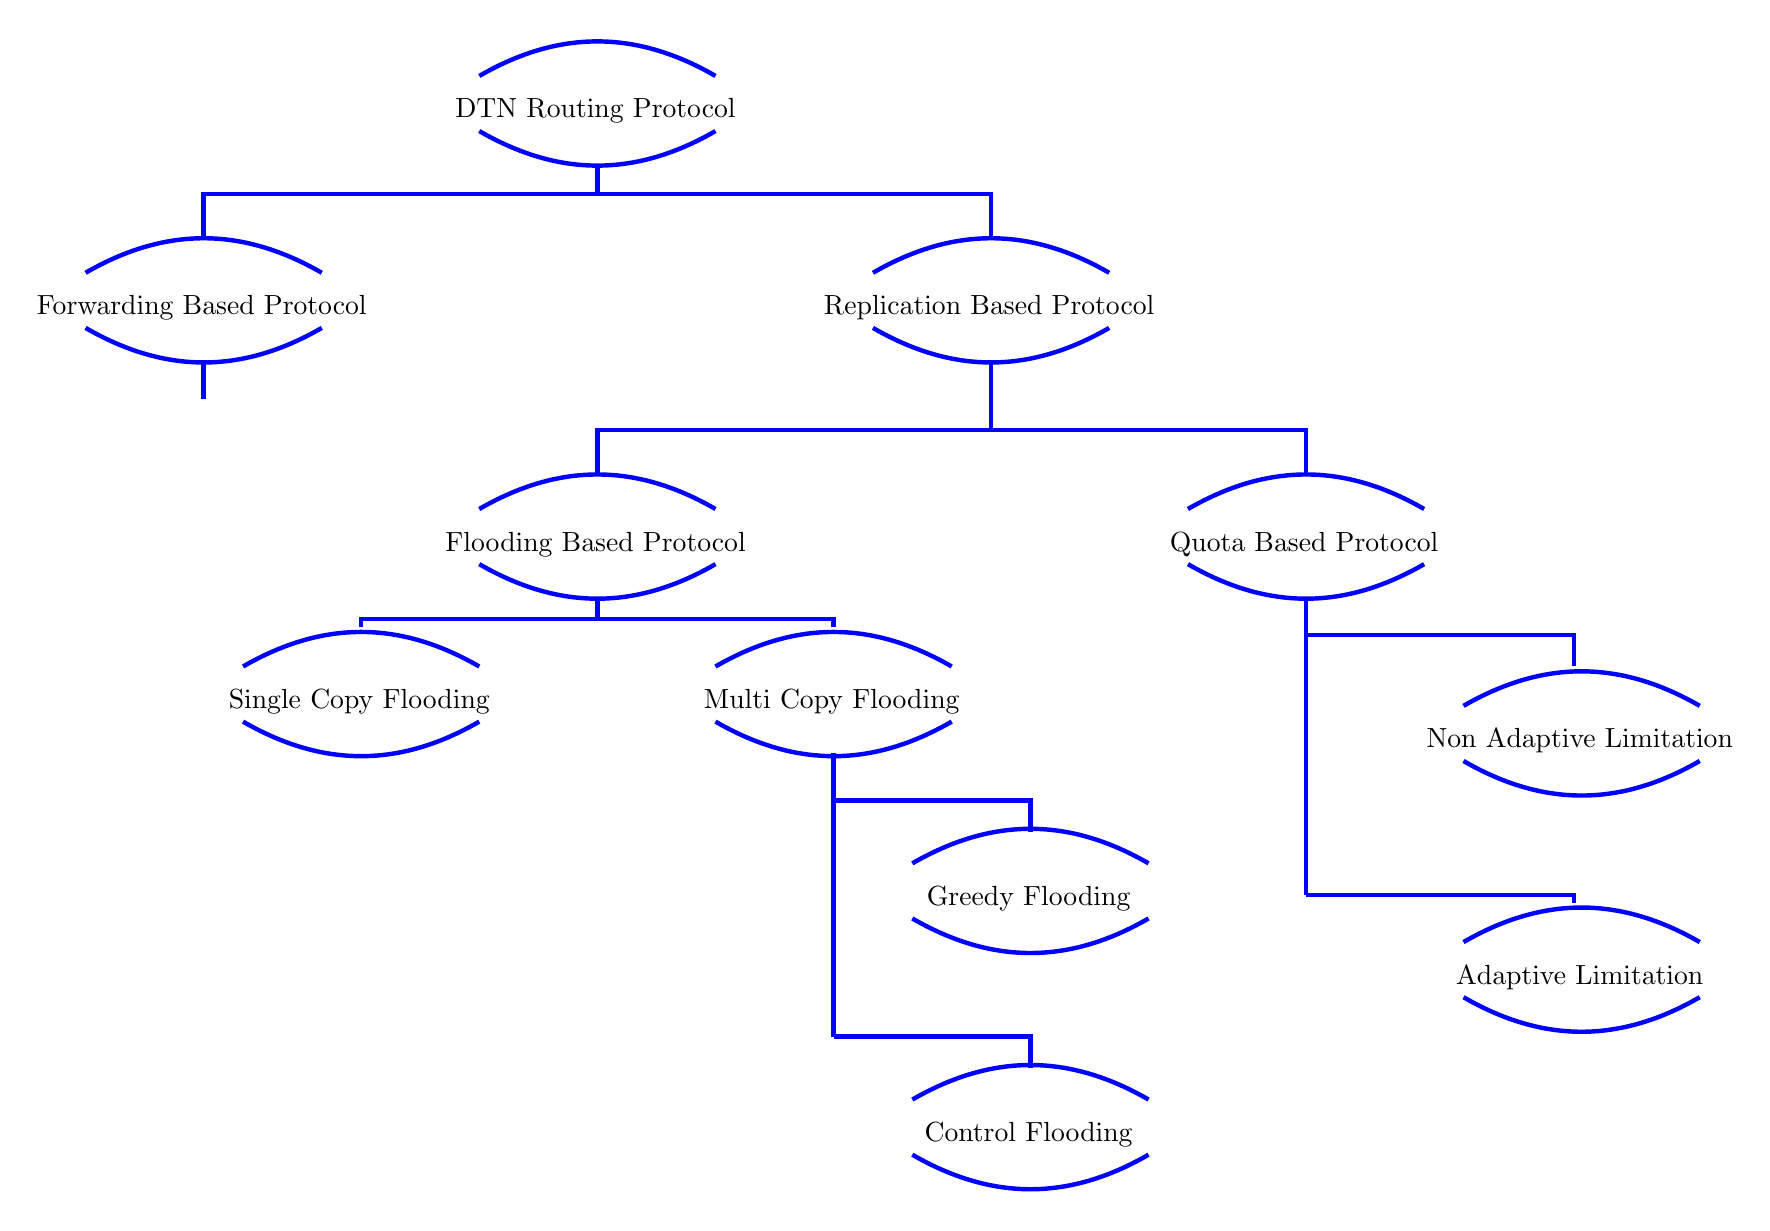
\begin{tikzpicture}

{[xshift=1.5cm,yshift=4cm]
    \draw[ultra thick,color=blue] node[auto,black,fill =white,xshift=4.2em,yshift=3em] {DTN Routing Protocol} (0,1.5) to [bend left](3,1.5);
    \draw[ultra thick,color=blue] (0,0.8) to[bend right] (3,0.8);
}

{[xshift=6.5cm,yshift=1.5cm]
    \draw[ultra thick,color=blue] node[auto,black,fill =white,xshift=4.2em,yshift=3em] {Replication Based Protocol} (0,1.5) to[bend left](3,1.5);
    \draw[ultra thick,color=blue] (0,0.8) to[bend right] (3,0.8);
}
{[xshift=10.5cm,yshift=-1.5cm]
    \draw[ultra thick,color=blue] node[auto,black,fill =white,xshift=4.2em,yshift=3em] {Quota Based Protocol} (0,1.5) to[bend left](3,1.5);
    \draw[ultra thick,color=blue] (0,0.8) to[bend right] (3,0.8);
}

{[xshift=14cm,yshift=-4cm]
    \draw[ultra thick,color=blue] node[auto,black,fill =white,xshift=4.2em,yshift=3em] {Non Adaptive Limitation} (0,1.5) to[bend left](3,1.5);
    \draw[ultra thick,color=blue] (0,0.8) to[bend right] (3,0.8);
}
{[xshift=14cm,yshift=-7cm]
    \draw[ultra thick,color=blue] node[auto,black,fill =white,xshift=4.2em,yshift=3em] {Adaptive Limitation} (0,1.5) to[bend left](3,1.5);
    \draw[ultra thick,color=blue] (0,0.8) to[bend right] (3,0.8);
}

{[xshift=1.5cm,yshift=-1.5cm]
    \draw[ultra thick,color=blue] node[auto,black,fill =white,xshift=4.2em,yshift=3em] {Flooding Based Protocol} (0,1.5) to[bend left](3,1.5);
    \draw[ultra thick,color=blue] (0,0.8) to[bend right] (3,0.8);
}
{[xshift=-1.5cm,yshift=-3.5cm]
    \draw[ultra thick,color=blue] node[auto,black,fill =white,xshift=4.2em,yshift=3em] {Single Copy Flooding} (0,1.5) to[bend left](3,1.5);
    \draw[ultra thick,color=blue] (0,0.8) to[bend right] (3,0.8);
}
{[xshift=4.5cm,yshift=-3.5cm]
    \draw[ultra thick,color=blue] node[auto,black,fill =white,xshift=4.2em,yshift=3em] {Multi Copy Flooding} (0,1.5) to[bend left](3,1.5);
    \draw[ultra thick,color=blue] (0,0.8) to[bend right] (3,0.8);
}
{[xshift=7cm,yshift=-6cm]
    \draw[ultra thick,color=blue] node[auto,black,fill =white,xshift=4.2em,yshift=3em] {Greedy Flooding} (0,1.5) to[bend left](3,1.5);
    \draw[ultra thick,color=blue] (0,0.8) to[bend right] (3,0.8);
}
{[xshift=7cm,yshift=-9cm]
    \draw[ultra thick,color=blue] node[auto,black,fill =white,xshift=4.2em,yshift=3em] {Control Flooding} (0,1.5) to[bend left](3,1.5);
    \draw[ultra thick,color=blue] (0,0.8) to[bend right] (3,0.8);
}
{[xshift=-3.5cm,yshift=1.5cm]
    \draw[ultra thick,color=blue] node[auto,black,fill =white,xshift=4.2em,yshift=3em] {Forwarding Based Protocol} (0,1.5) to[bend left](3,1.5);
    \draw[ultra thick,color=blue] (0,0.8) to[bend right] (3,0.8);
}
    {[xshift=3cm,yshift=3.5cm]\draw[ultra thick,color=blue] (0,0.47) to (0,0.85);} %DTNRouting
{[xshift=3cm,yshift=3cm]    \draw[ultra thick,color=blue] (0,1) -| (5,0.45);}

{[xshift=3cm,yshift=3cm]    \draw[ultra thick,color=blue] (-0,1) -| (-5,0.45);}

{[xshift=8cm,yshift=1cm]\draw[ultra thick,color=blue] (0,0) to (0,0.85);} %Replication
{[xshift=8cm,yshift=-0cm]    \draw[ultra thick,color=blue] (0,1) -| (4,0.45);}

{[xshift=8cm,yshift=-0cm]    \draw[ultra thick,color=blue] (-0,1) -| (-5,0.45);}

{[xshift=-2cm,yshift=1cm]\draw[ultra thick,color=blue] (0,0.4) to (0,0.85);} %Fowarding
{[xshift=3cm,yshift=-2cm]\draw[ultra thick,color=blue] (0,0.6) to (0,0.85);} %Flooding
{[xshift=3cm,yshift=-2.4cm]    \draw[ultra thick,color=blue] (0,1) -| (3,0.9);}
{[xshift=3cm,yshift=-2.4cm]    \draw[ultra thick,color=blue] (0,1) -| (-3,0.9);}


{[xshift=12cm,yshift=-2cm]\draw[ultra thick,color=blue] (0,0.4) to (0,0.85);} %Qouta Based
{[xshift=12cm,yshift=-2.6cm]    \draw[ultra thick,color=blue] (0,1) -| (3.4,0.6);}
{[xshift=12cm,yshift=-2.5cm]\draw[ultra thick,color=blue] (0,-2.4) to (0,0.9);}
{[xshift=12cm,yshift=-5.9cm]    \draw[ultra thick,color=blue] (0,1) -| (3.4,0.9);}
{[xshift=6cm,yshift=-4cm]\draw[ultra thick,color=blue] (0,0.4) to (0,0.85);} %Multi
{[xshift=6cm,yshift=-4.7cm]    \draw[ultra thick,color=blue] (0,1) -| (2.5,0.6);}
{[xshift=6cm,yshift=-4cm]\draw[ultra thick,color=blue] (0,-2.7) to (0,0.9);}
{[xshift=6cm,yshift=-7.7cm]    \draw[ultra thick,color=blue] (0,1) -| (2.5,0.6);}
\end{tikzpicture}

%\setlength{\unitlength}{.5mm}
%\begin{picture}(120, 168)
%\newsavebox{\foldera}%           declaration
%\savebox{\foldera}(40, 32)[l]{%  definition
%  \multiput(0, 0)(0, 28){2}{\line(1, 0){40}}
%  \multiput(0, 0)(40, 0){2}{\line(0, 1){28}}
%  \put(1, 28){\oval(2, 2)[tl]}
%  \put(1, 29){\line(1, 0){5}}
%  \put(9, 29){\oval(6, 6)[tl]}  
%  \put(9, 32){\line(1, 0){8}}
%  \put(17, 29){\oval(6, 6)[tr]}
%  \put(20, 29){\line(1, 0){19}}
%  \put(39, 28){\oval(2, 2)[tr]}
%}
%\newsavebox{\folderb}%           declaration      
%\savebox{\folderb}(40, 32)[l]{%  definition
%  \put(0, 14){\line(1, 0){8}}
%  \put(8, 0){\usebox{\foldera}}
%}
%\multiput(0, 0)(120, 0){2}{\line(0, 1){168}}
%\multiput(0, 0)(0, 168){2}{\line(1, 0){120}}
%\put(34, 26){\line(0, 1){102}}
%\put(14, 128){\usebox{\foldera}}
%\multiput(34, 86)(0, -37){3}{\usebox{\folderb}}
%\end{picture}
%\begin{tikzpicture}
%\matrix[nodes={draw, fill=blue!20},
%    row sep=0.3cm,column sep=0.3cm,minimum width=.875cm, minimum height=1cm] {
%    \node[ellipse callout] {Callouts}; & \node [cylinder] {C}; &
%    %
%    \node [arrow box] {A};\\
%    %
%    \node[rectangle split, rectangle split parts=3, draw, text width=2.75cm]
%        {Student
%        \nodepart{second}
%        age:int \\
%        name:String
%        \nodepart{third}
%        getAge():int \\
%        getName():String}; &
%    %
%    \node[nor gate IEC, draw, logic gate inputs=in] (A) {};
%    \draw (A.input 1 -| -1,0) -- (A.input 1) (A.input 2 -| -1,0) -- (A.input 2)
%        (A.output) -- ([xshift=0.5cm]A.output); &
%    %
%    \node[or gate US, draw,logic gate inputs=inini] (A) {};
%    \foreach \a in {1,...,5}
%        \draw (A.input \a -| -1,0) -- (A.input \a);
%        \draw (A.output) -- ([xshift=0.5cm]A.output);\\
%};
%\end{tikzpicture}
%
%\begin{tikzpicture}[inner sep=0pt,thick,
%    dot/.style={fill=blue,circle,minimum size=3pt}]
%    \draw[help lines] (0,0) grid (3,2);
%    \node[dot] (a) at (1,1) {};
%    \node[dot] (b) at (2,2) {};
%    \node[dot] (c) at (1,2) {};
%    \node[dot] (d) at (1.25,0.25) {};
%    \node[dot] (e) at (1.75,1.5) {};
%    \node[draw=red, fit=(a) (b) (c) (d) (e)] {box};
%    \node[draw,circle,fit=(a) (b) (c) (d) (e)] {};
%\end{tikzpicture}
%
%\begin{tikzpicture}
%    \node[starburst,drop shadow,fill=white,draw] {Drop shadow};
%    \node[copy shadow,fill=blue!20,draw=blue,thick] at (3.5,0) {Copy shadow};
%    \node[circle,circular drop shadow,fill=blue!20,draw] at (6,0) {Circular};
%\end{tikzpicture}
%
%\begin{tikzpicture}[every on chain/.style=join,every join/.style=->,
%    node distance=2mm and 1cm]
%    { [start chain=trunk]
%        \node [on chain] {A};
%        \node [on chain] {B};
%        { [start branch=numbers going below] } % just a declaration,
%        { [start branch=greek going above] } % we will come back later
%        \node [on chain] {C};
%        % Now come the branches...
%        { [continue branch=numbers]
%            \node [on chain] {1};
%            \node [on chain] {2};
%        }
%        { [continue branch=greek]
%            \node [on chain] {$\alpha$};
%            \node [on chain] {$\beta$};
%        }
%    }
%\end{tikzpicture}
%
%\begin{tikzpicture}
%    % Checker board
%    \fill [black!20] (-1.5,-1.5) rectangle (3.5,1.5);
%    \pattern [pattern=checkerboard,pattern color=black!30]
%        (-1.5,-1.5) rectangle (3.5,1.5);
%    \node at (0,0) [opacity=0.5,forbidden sign,line width=2ex,
%        draw=red,fill=white]
%        {Smoking};
%    \begin{scope}[opacity=.5,transparency group]
%        \node at (2,0) [forbidden sign,line width=2ex,draw=red,fill=white]
%        {Smoking};
%    \end{scope}
%    \begin{scope}[xshift=4cm,yshift=-1.5cm,path fading=south]
%        % Checker board
%        \fill [black!20] (0,0) rectangle (4,3);
%        \pattern [pattern=checkerboard,pattern color=black!30]
%            (0,0) rectangle (4,3);
%        \fill [color=blue] (0.5,1.5) rectangle +(1,1);
%        \fill [color=blue,path fading=north] (2.5,1.5) rectangle +(1,1);
%        \fill [color=red,path fading] (1,0.75) ellipse (.75 and .5);
%        \fill [color=red] (3,0.75) ellipse (.75 and .5);
%    \end{scope}
%\end{tikzpicture}
%
%\begin{tikzpicture}[every node/.style=draw]
%    \draw[help lines] (0,0) grid (2,2);
%    \node (some node) at (1,1) {some node};
%    \node (other node) [above=1cm of some node] {\tiny above=1cm of some node};
%    \draw [<->] (some node) -- (other node)
%    node [midway,right,draw=none] {1cm};
%
%    \node (X) at (0,0) {X};
%    \node (a) [base right=0.5cm of X ] {a};
%    \node (y) [base right=of a] {y};
%\end{tikzpicture}
%
%\begin{tikzpicture}
%    { []
%        \draw [help lines] (0,0) grid (3,2);
%        \coordinate (a) at (1,0);
%        \coordinate (b) at ($(a)+1/2*(3,3)$);
%        \draw (a) -- (b);
%        \coordinate (c) at ($ (a)!.25!(b) $);
%        \coordinate (d) at ($ (c)!1cm!90:(b) $);
%        \draw [<->] (c) -- (d) node [sloped,midway,above] {1cm};
%    }
%    { [xshift=4cm]
%        \draw [help lines] (0,0) grid (3,2);
%        \coordinate (a) at (0,1);
%        \coordinate (b) at (3,2);
%        \coordinate (c) at (2.5,0);
%        \draw (a) -- (b) -- (c) -- cycle;
%        \draw[red] (a) -- ($(b)!(a)!(c)$);
%        \draw[orange] (b) -- ($(a)!(b)!(c)$);
%        \draw[blue] (c) -- ($(a)!(c)!(b)$);
%    }
%\end{tikzpicture}
%
%
%\begin{tikzpicture}
%    { []
%        \draw[help lines] (0,0) grid (3,2);
%        \draw
%            [preaction={draw,line width=4mm,blue}]
%            [line width=2mm,red] (0,0) rectangle (2,2);
%    }
%    { [xshift=4cm]
%
%        \draw[help lines] (0,0) grid (3,2);
%        \draw
%            [postaction={draw,line width=2mm,blue}]
%            [line width=4mm,red,fill=white] (0,0) rectangle (2,2);
%    }
%\end{tikzpicture}


\end{document}